\section{Evaluation}
\label{sec:evaluation}

We prove the correctness and liveness of \sys in Appendix~\ref{appx:proof}. Our evaluation centers around five aspects:

\parab{Scalable throughput.}\sys achieves throughput close to underlying hardware limit (8M messages per second), and scales linearly to 1K hosts.

\parab{Low latency.}With reconfigurable chip, \sys adds less than 5$\mu$s to one-way delay for 1K hosts. With switch CPU, \sys adds less than 15$\mu$s delay.

\parab{Low bandwidth and computation overhead.}In our settings, \sys consumes 0.1\% bandwidth on idle network links, and adds an 8-byte tag to each network packet. At switches, beacon packets can be processed by a CPU core. At hosts, reordering computation consumes less than 10\% of a core.

\parab{Fault tolerance.}When a host, switch or link fails, non-failure nodes resumes normal throughput and latency in a beacon timeout (1ms). When a node recovers from failure, it can join the system in one RTT (10$\mu$s).

\parab{Background traffic.}\sys is adaptive to delay variance in the network and the clocks are re-synchronized for every beacon interval. Hence, \sys can share the network fairly with background TCP traffic.

\subsection{Methodology}
\label{sec:testbed}

We build two testbeds in two data centers.
The first one has 3 servers connected to a Barefoot Tofino 100G switch~\cite{tofino}.
The second one has 8 servers and 4 Arista 7060CX 100G switches~\cite{arista}, forming a fat-tree topology.
Each server has two Xeon E5 CPUs and one Mellanox ConnectX-4 NIC running RoCEv2~\cite{infinibandrocev2}.

%We use a testbed of 8 Dell R720/R730 servers and 10 Arista 100G Ethernet switches~\cite{arista} to benchmark the efficiency of \sys. %The topology is similar to Figure~\ref{fig:dcn}.
%Each server is equipped with two Xeon E5 CPUs and one Mellanox ConnectX-4 NIC. Because we have not found a low latency interface in the switch OS to process beacon packets, we connect one Dell R720 server with Mellanox ConnectX-3 NICs to each of the switches to mimic the switch CPU. %Since the bottleneck in our benchmarks is the CPU instead of the network, there is unlikely to be congestion loss.
%Performance using data-plane programmable switches are expected to be better, but not evaluated because we do not have such a switch.

In small-scale experiments (1$\sim$8 hosts), each server uses a pair of dedicated cores for sending and receiving, respectively.
For experiments with 16$\sim$128 hosts, we use each physical server as 16 logical servers. Each logical server has a pair of dedicated cores, maintains timestamps independently and communicates via separate RDMA queue pairs.
To evaluate datacenter-scale scalability ($\ge$256 hosts), we build a simple simulator.
We choose beacon interval to be 10~$\mu$s.


\iffalse
\begin{table}[t]
\centering
\scalebox{0.85}{
\begin{tabular}{|l|r|r|r|r|r|r|}
\hline
Servers & \multicolumn{3}{c|}{Num switches} & \multicolumn{3}{c|}{Num downlinks} \\
\hline
Host & ToR & Leaf & Core & ToR & Leaf & Core \\
\hline
2        & 1 & 0 & 0 & 2 & 0 & 0 \\
\hline
4    & 2 & 2 & 0 & 2 & 2 & 0 \\
\hline
8    & 4 & 4 & 2 & 2 & 2 & 4 \\
\hline
64    & 8 & 4 & 2 & 8 & 4 & 4 \\
\hline
1024  & 64 & 16 & 8 & 16 & 16 & 16 \\
\hline
\end{tabular}
\vspace{-10pt}
}
\caption{Network topologies for evaluation.}
\label{tab:eval-topology}
\end{table}

We evaluate 5 different system scales in Table~\ref{tab:eval-topology}: testbed consisting of one to three layers of network switches, as well as simulation of three-layer fat-tree topology with 64 or 1024 hosts.
Topologies in Table~\ref{tab:eval-topology}.
For large-scale experiments, we use NS-3~\cite{henderson2008network} for simulation.
The link bandwidth, link delay and processing delay are extracted from three-layer testbed experiments.
To make simulations faster, each sender only sends one message to a randomly chosen receiver.
\fi

\subsection{Scalability and Efficiency}

\begin{figure*}[t]
        \begin{minipage}[t]{.32\textwidth}
                \centering
                \subfloat[Throughput]{
                        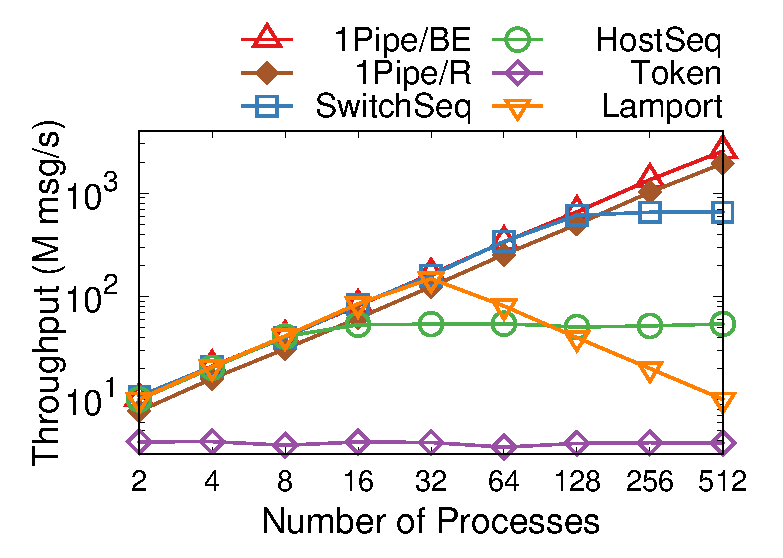
\includegraphics[width=\textwidth]{gnuplot/total_order.eps}
                }
                \newline
                \subfloat[Latency]{
                        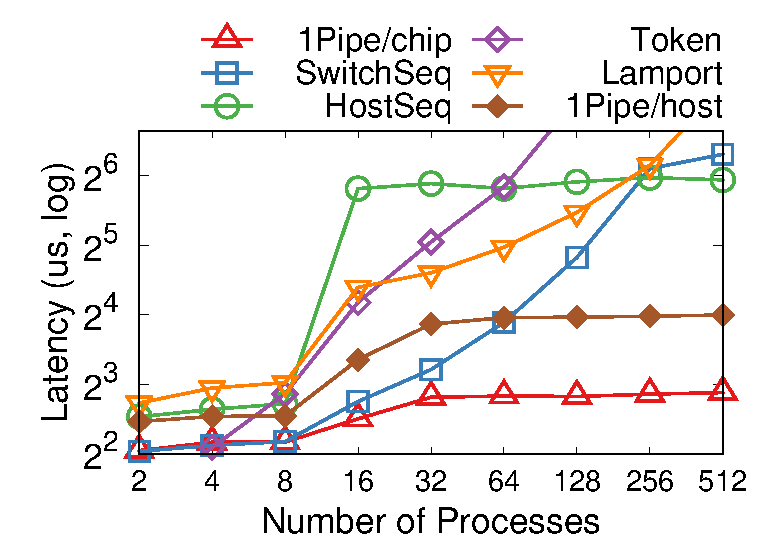
\includegraphics[width=\textwidth]{gnuplot/total_order_lat.eps}
                }
                \caption{Scalability comparison of total order algorithms.}
                \label{fig:total-order}
        \end{minipage}
        \hspace{0.01\textheight}
        \begin{minipage}[t]{.32\textwidth}
                \centering
                \subfloat[Reconfigurable switch (P4 switch), fixed-function switch (switch CPU) or end hosts.\label{fig:reorder-testbed}]
                {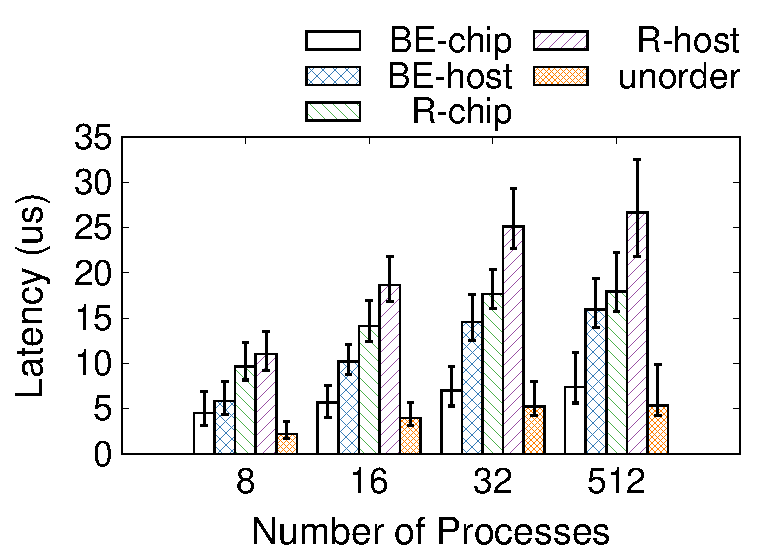
\includegraphics[width=\textwidth]{gnuplot/reorder_testbed.eps}}
                \newline
                \subfloat[Simulation with different end-host delays.
                T-R\textit{i} shows minimax clock synchronization, P-R\textit{i} shows physical clock synchronization.\label{fig:reorder-simulation}]
                {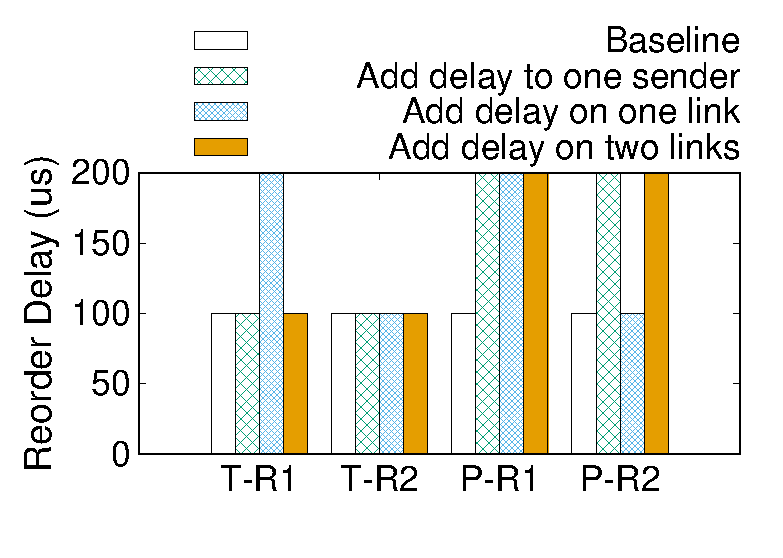
\includegraphics[width=\textwidth]{gnuplot/reorder_simulation.eps}}
                \caption{Average reordering delay.}
                \label{fig:reorder-delay}
        \end{minipage}
        \hspace{0.01\textwidth}
        \begin{minipage}[t]{.32\textwidth}
                \centering
                \subfloat[Network bandwidth overhead.\label{fig:network-overhead}]
                {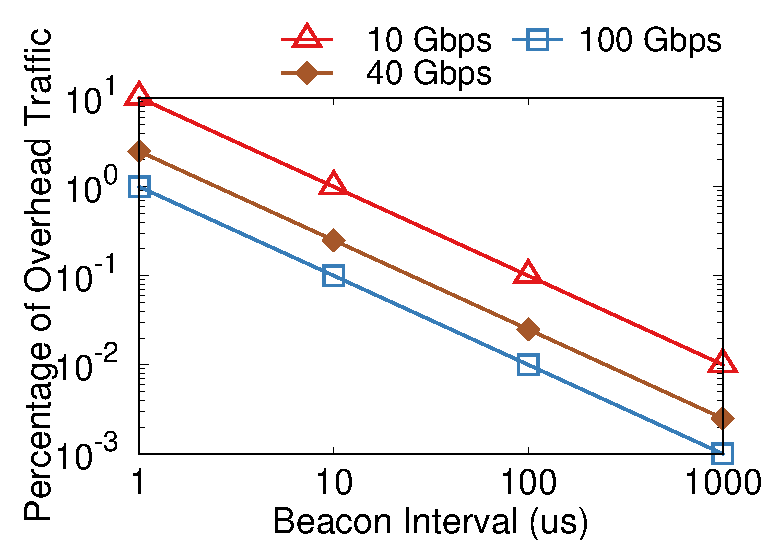
\includegraphics[width=\textwidth]{gnuplot/beacon_network_overhead.eps}}
                \newline
                \subfloat[CPU processing overhead.\label{fig:cpu-overhead}]
                {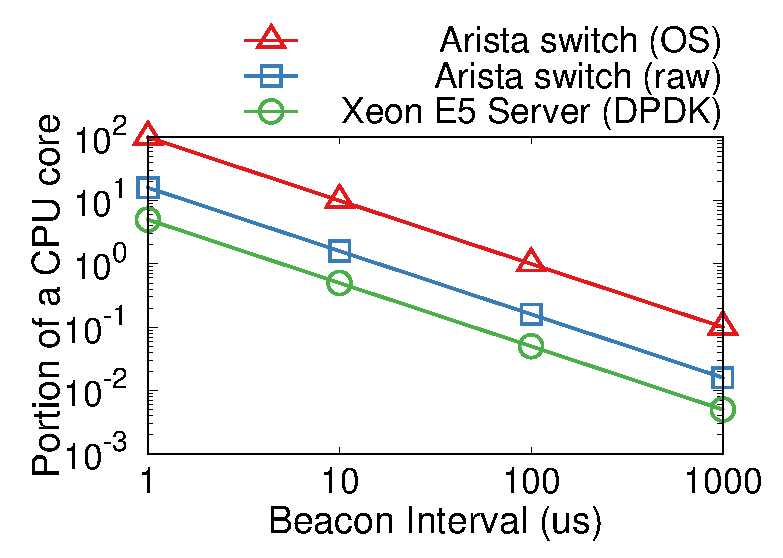
\includegraphics[width=\textwidth]{gnuplot/beacon_cpu_overhead.eps}}
                \caption{
                        Beacon overhead under different beacon intervals and network throughput.
                        CPU processing overhead for Arista switch is extrapolated.
                }
                \label{fig:overhead}
        \end{minipage}
\vspace{-1.6em}
\end{figure*}

\subsubsection{Scalability of Total Ordering}

Figure~\ref{fig:total-order} compares the scalability of \sys with other total order multicast algorithms using centralized sequencer~\cite{eris,kaminsky2016design}, token~\cite{rajagopalan1989token}, ISIS~\cite{birman1985replication} and Lamport timestamp~\cite{lamport1978time}. The throughput of \sys is limited by CPU processing and RDMA messaging rate (8~M messages per second per core).
It scales almost linearly to 128 hosts in the testbed and 1K hosts in simulation.
Although recent advances in RDMA~\cite{kaminsky2016design} and programmable switches~\cite{eris} make sequencers fast, it is still a central bottleneck and introduces extra network delay.
In timestamp-based ordering, a receiver waits for timestamps from other receivers before delivery, introducing delivery delay as well as network overhead.




\subsubsection{Reordering Delay}
\label{sec:eval-delay}

Figure~\ref{fig:reorder-testbed} shows the average reordering delay of \sys.
Reordering delay is the time from receiving a message to delivering it.
Using end host representatives to process beacons introduces additional delay due to forwarding delay from the switch to the end host representatives.
As the number of network layers increases, the reordering delay increases, due to beacon processing delay at each switch.
\RED{The beacon interval is not amplified by network layers, because the algorithm synchronizes beacon arrival times. doesn't make sense}
For three-layer topology, the number of hosts adds slightly to reordering delay, because a switch with higher fan-out is likely to have more skew in beacon synchronization.

Figure~\ref{fig:reorder-simulation} shows how minimax clock synchronization adapts to imbalanced link or host delays.
We simulate two senders and two receivers connected via 4 links.
When one sender $S_1$ has 10~$\mu$s more delay due to background traffic, minimax clock synchronization adjusts the sender's timestamp to preserve minimal reordering delay, while physical clock synchronization does not account for the different sender delays.
When one network link $S_2 \rightarrow R_2$ has 100~$\mu$s more delay, due to multipath, both synchronization mechanisms have more reordering delay.\RED{maximum delay in Figure~\ref{fig:reorder-simulation} is 20us, not 100us}
When two links $S_2 \rightarrow R_1$ and $S_2 \rightarrow R_2$ both have 10~$\mu$s more delay, minimax clock synchronization can compensate the change.



%\begin{figure}[t]
%\centering
%
\includegraphics[width=0.48\textwidth]{images/fixme.pdf}
%\caption{CDF of end-to-end delay and reordering delay.}
%\label{fig:cdf-delay}
%\end{figure}


\subsubsection{Network Overhead}
\label{sec:eval-overhead}

Beacons are network packets that consume bandwidth.
As shown in Figure~\ref{fig:network-overhead}, under high speed networks and a reasonable beacon interval, the beacon traffic is a tiny portion of available link bandwidth.
Because beacons are hop-by-hop, the overhead is only related to beacon interval and does not change with system scale.

\subsubsection{CPU Overhead}
\label{sec:eval-cpu-overhead}

The CPU overhead of \sys has two parts: beacon processing on switches and reordering on receivers.
Figure~\ref{fig:cpu-overhead} shows the number of cores required for beacon processing of a 32-port switch.
The Arista switch has 4 CPU cores.
The raw packet processing capacity of a switch CPU core is 1/3 of a Xeon E5 CPU core.
If we are able to bypass the kernel network stack and process packets efficiently in Arista switches, a single switch CPU core can sustain 10~$\mu$s beacon interval.

As shown in Figure~\ref{fig:reorder-overhead}, although the maximal buffer size required on the receiver increases linearly with beacon interval, the message reordering throughput of a CPU core does not degrade significantly.


Figure~\ref{fig:clock-sync} compares reordering delay of minimax clock synchronization with physical clock synchronization (PTP).

\subsection{Deep Dive}


Then we deep dive into the behavior of \sys under packet loss, failure and incremental deployment.

\begin{table}
\centering
\scalebox{0.9}{
\begin{tabular}{l|r|r|r|r}
        \hline
         & $S_1 \rightarrow R_1$ & $S_1 \rightarrow R_2$ & $S_2 \rightarrow R_1$ & $S_2 \rightarrow R_2$ \\
    \hline
    \hline
    $S_1$ fail & N/A & N/A & $T_{timeout}$ & $T_{timeout}$ \\
    \hline
    $S_1$ recover & RTT & RTT & 0 & 0 \\
    \hline
    $R_1$ fail & N/A & $T_{timeout}$ & N/A & $T_{timeout}$ \\
    \hline
    $R_1$ recover & RTT & 0 & RTT & 0 \\
    \hline
    $SW_1$ fail & $T_{timeout}$ & $T_{timeout}$ & $T_{timeout}$ & $T_{timeout}$ \\
    \hline
    $SW_1$ recover & 0 & 0 & 0 & 0 \\
    \hline
\end{tabular}
}
\caption{
        Convergence time after failure and recovery of host and switch.
        Convergence time is the time since the event occurs until end-to-end delay recovers to normal.
    Convergence time 0 indicates not affected.
    $T_{timeout}$ is the beacon timeout for failure detection.
}
\label{tab:failure}
\end{table}

We consider a network with two senders $S_1, S_2$, two receivers $R_1, R_2$ interconnected via two switches $SW_1, SW_2$.
Each switch is connected to all four hosts.
Table~\ref{tab:failure} shows how long a failure or recovery would impact the system.

Figure~\ref{fig:background-flow} shows the reordering delay when a background flow is inserted. \RED{Should be removed as well?}


\iffalse
\subsubsection{Incremental Deployment}
\label{sec:eval-incremental}


\begin{figure}[t]
\centering
        \subfloat[Clock convergence.\label{fig:clock-convergence}]
        {
\includegraphics[width=.23\textwidth]{images/fixme.pdf}}
        \hspace{0.01\textwidth}
        \subfloat[Reordering delay.\label{fig:incremental-delay}]
        {
\includegraphics[width=.23\textwidth]{images/fixme.pdf}}
\caption{[Simulation] Merging two running TOMS systems by adding a network link between them.}
\label{fig:incremental}
\end{figure}

Figure~\ref{fig:clock-convergence} shows
Converge time graph, compare with physical time synchronization solution

Figure~\ref{fig:incremental-delay} shows the reordering delay. (spike then fall back)
\fi
